\def\theTopic{Reading 17}

\begin{center}
{\bf {\large From Dots to ``Dust''}}
\end{center}


Recall the definition of a p-value:

{\sf The probability of observing results this extreme or more extreme
  if $H_0$ is true}

The idea of probability is of great importance in statistics.\\
To compute probabilities, we have run a simulation (assuming $H_0$ is
true), counted dots in the extremes, then divided by the number of
simulations to get an approximate p-value.

Similarly, for confidence intervals:  We have counted from the outside
in to have a certain number of dots outside the interval, and inside,
the number of dots divided by the total number matched the confidence
level.  


We have  seen that we get better accuracy for p-values (and
probabilities in general) if we run large numbers of simulations.
Suppose we are looking at a single mean. What happens as we increase
the number of simulations?
\begin{itemize}
  \item Our dots need to get smaller to fit into the graph.
  \item The outline of the distribution will get smoother.
\end{itemize}

The title of this page comes from the idea that we can increase the
number of dots and decrease their size, until they are like ``dust''. 
The lumpiness of the distribution will also smooth out till we get a
smoother curve across the top of the dots.

In Unit 3 we will use smooth curves instead of dots to
compute probabilities. You need to keep these ideas in mind:
\begin{itemize}
  \item To compute probability for a given interval, take the area
    under the curve over that interval.
  \item The area under the entire curve is exactly 1.
\end{itemize}


As a simple example, we could have a ``curve'' which is zero for
values less than 0 or greater than 10, and jumps up to a constant
value between 0 and 10.  That is not ``curved'', but it does fit the
definition if we pick the right ``y'' value for the constant value
between 0 and 10.  What constant must we use to make the area under
this ``curve'' be 1? 


Label the y axis ticks to show the value at the top. 

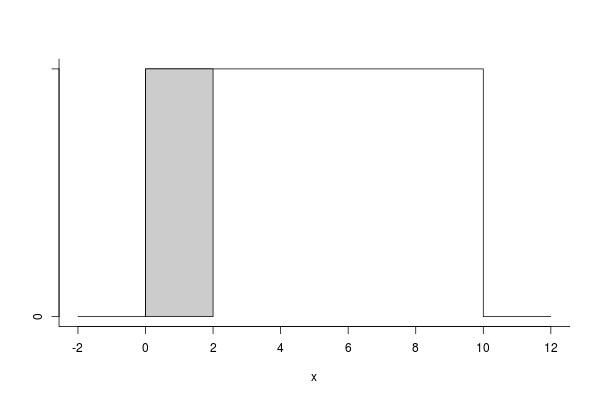
\includegraphics[width=.6\linewidth]{plots/uniformDensity0-10.png}

% x <- c(-2,-0.0001,0,10,10.0001,12)
% plot(x, dunif(x,0,10),  ylab = "", yaxt = "n", type = "l")
% rect(0,0,2,.1, col = grey(.8))
% axis(side=2, at = 0:1/10, labels = c(0,""))
% dev.copy(png, file = "plots/uniformDensity0-10.png",height=400,width = 600);dev.off(

If the area under the whole curve is 1, what is the area of the shaded rectangle?\\

In the plot below is another probability curve. What area is shaded?

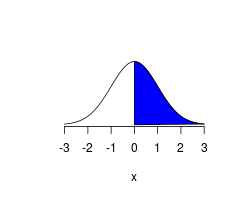
\includegraphics[width=.4\linewidth]{../plots/halfNormal.png}


\begin{center}
  {\large\bf Important Points}
\end{center}

\begin{itemize}
\item Curves are often used to represent probability
  distributions. The area under the whole curve must be one.
\item The connection between the dots we've been using and the curve
  is to imagine that we sample from the distribution a huge
  number of times. The dots we have been plotting would then have to
  each take up a very tiny space (like a dust mote), and instead of
  counting dots, we could just measure their area.
\item The total area under a probability density curve is one.
\item The probability of drawing a number from some interval is the
  area above the interval and under the curve.  Even a rectangle can
  be considered a ``curve''.
\end{itemize}
